\documentclass[10pt,a4paper]{article}
\usepackage[utf8]{inputenc}
\usepackage[T1]{fontenc}
\usepackage[brazil]{babel}
\usepackage[margin=1.7cm]{geometry}
\usepackage{booktabs}
\usepackage{enumitem}
\usepackage{microtype}
\usepackage{graphicx}
\usepackage{xcolor}
\usepackage{tikz}
\newcommand{\tikzmark}[1]{\tikz[overlay,remember picture,baseline=0pt]\node[inner sep=0pt,outer sep=0pt] (#1) at (0,0) {};}
\usepackage[font=small,labelfont=bf]{caption}

\setlength{\parindent}{0pt}
\setlength{\parskip}{3pt}
\setlist{nosep,leftmargin=1.2em}
\pagestyle{empty}

\title{\vspace{-1.4cm}\textbf{Relat\'orio: An\'alise de Fairness no Sistema de Cr\'edito}\\[2pt]
\normalsize \'Etica em Intelig\^encia Artificial --- Toolkit de Bias e Fairness (Parte 3/3)\vspace{-0.4cm}}
\author{\small Jefferson Cunha --- \texttt{jefferson.cunha@ufpe.br}\\[1pt]
\small Disciplina: \'Etica e Intelig\^encia Artificial --- 2\textsuperscript{o} sem/2026 --- Prof.\ Geber Ramalho}
\date{\vspace{-0.6cm}}

\begin{document}
\maketitle

\textbf{Metodologia.} Simulei 2000 clientes (60\% homens, 40\% mulheres; \texttt{seed}=42). O \textit{score} base combina renda, \textit{score} de cr\'edito, raz\~ao d\'ivida/renda e idade. Para mulheres, o \textit{score} \'e multiplicado por \texttt{VIES\_GENERO}. A decis\~ao \'e \texttt{score > threshold}, e o \textit{ground truth} \'e \texttt{score\_base > 0,5}. DPD = $|$taxa$_H$ $-$ taxa$_M|$.

\section*{1. Sem vi\'es e com vi\'es forte}
Com \texttt{VIES\_GENERO} = 1,0 h\'a diferen\c{c}a pequena (homens 85,9\%, mulheres 82,4\%; DPD 0,035), devida \`a variabilidade amostral. Com 0,8, as mulheres caem para 34,2\% e a diferen\c{c}a chega a \textbf{51,7 p.p.}. O DPD mede o quanto o resultado depende do grupo, sem olhar se a decis\~ao estava correta. Detalhes no Ap\^endice~A.1.

\section*{2. Thresholds diferentes}
Com \texttt{THRESHOLD\_MULHERES} = 0,45: no \textit{notebook} (vi\'es 1,0) o DPD piora (0,035 $\to$ 0,087) e a acur\'acia cai de 100\% para 95,2\%; com vi\'es 0,8 o DPD cai (0,517 $\to$ 0,250) e a acur\'acia sobe (80,8\% $\to$ 91,5\%). A melhor combina\c{c}\~ao (homens 0,50; mulheres \textbf{0,39}) d\'a DPD 0,007 e acur\'acia 98,4\%; o ``pre\c{c}o'' de fairness $\approx$ perfeita \'e de s\'o \textbf{1,6 p.p.}\ de acur\'acia (Ap\^endice~A.2).

\section*{3. Reflex\~oes \'eticas e pr\'aticas}
\begin{itemize}
  \item \textbf{Thresholds diferentes por g\^enero s\~ao \'eticos?} \'E uma quest\~ao complexa. Pela \textit{equidade de resultados} (paridade demogr\'afica), ajustar thresholds corrige distor\c{c}\~oes sist\^emicas e promove justi\c{c}a compensat\'oria. Mas, no Brasil (LGPD, princ\'ipio da n\~ao discrimina\c{c}\~ao, art.~6\textsuperscript{o}, IX) e nos EUA (\textit{Equal Credit Opportunity Act}), usar atributo protegido para aplicar regras distintas na concess\~ao de cr\'edito caracteriza tratamento discriminat\'orio direto. O ideal n\~ao \'e ``baixar a r\'egua'' no final, e sim corrigir vieses estruturais nos dados, remover vari\'aveis \textit{proxy} ou treinar com restri\c{c}\~oes de fairness, para que o modelo trate indiv\'iduos de forma igualit\'aria por constru\c{c}\~ao.
  \item \textbf{Outros fatores de vi\'es.} Algoritmos raramente usam g\^enero diretamente; o vi\'es se esconde em \textit{proxies}: hist\'orico de renda e emprego (pausas de carreira, licen\c{c}a-maternidade), CEP (ra\c{c}a e classe, vi\'es espacial), profiss\~ao/setor (setores feminizados com remunera\c{c}\~ao m\'edia distinta) e vi\'es de amostragem (hist\'orico de mais cr\'edito a homens leva o modelo a confiar mais no perfil masculino).
  \item \textbf{Explica\c{c}\~ao ao gerente focado em lucro.} Foco em risco de longo prazo e oportunidade perdida: (i) \textit{custo de oportunidade}, pois o modelo enviesado gera falsos negativos e rejeita boas pagadoras; (ii) \textit{risco regulat\'orio}, pois multas e auditorias custam mais que a pequena perda de acur\'acia; (iii) \textit{reputa\c{c}\~ao}, pois esc\^andalo de discrimina\c{c}\~ao afeta a marca e afasta clientes. Perder alguns pontos de acur\'acia \'e aceitar um risco um pouco maior de inadimpl\^encia (mais falsos positivos) para ampliar a base de clientes saud\'aveis e garantir conformidade. Na simula\c{c}\~ao, corrigir o vi\'es custou 1,6 p.p., e n\~ao corrigir custou 19,2 p.p.\ (100\% $\to$ 80,8\%).
\end{itemize}

\section*{4. \textit{Lessons learned}}
Os artigos apresentaram novidades quanto \`as diferentes categorias de vieses algor\'itmicos e mostraram, de forma material, que h\'a complexidade e implica\c{c}\~oes \'eticas na forma de resolv\^e-los: seja com a introdu\c{c}\~ao de compensadores ap\'os o resultado, o que implica reduzir a acur\'acia do modelo; seja, em contrapartida, pela aus\^encia de dados suficientes para compensar um treinamento menos enviesado.

\newpage
\section*{Ap\^endice A --- Detalhamento das Se\c{c}\~oes 1 e 2}
\subsection*{A.1 Sem vi\'es e com vi\'es forte (detalhe da Se\c{c}\~ao 1)}
\begin{itemize}
  \item \textbf{\texttt{VIES\_GENERO} = 1,0.} H\'a diferen\c{c}a pequena: homens 85,9\% e mulheres 82,4\% (DPD = 0,035). N\~ao h\'a vi\'es intencional; a diferen\c{c}a vem da \textbf{variabilidade amostral}. G\^enero \'e sorteado independentemente das \textit{features}, ent\~ao a diferen\c{c}a tende a zero com amostras maiores. A acur\'acia \'e 100\%, pois a decis\~ao coincide com o \textit{ground truth}.
  \item \textbf{\texttt{VIES\_GENERO} = 0,8.} Homens 85,9\% e mulheres 34,2\%: diferen\c{c}a de \textbf{51,7 pontos percentuais} (DPD $\approx$ 0,52). Mulheres t\^em taxa de aprova\c{c}\~ao 60\% menor, e a acur\'acia cai para 80,8\%.
  \item \textbf{DPD na pr\'atica.} \'E a diferen\c{c}a entre as taxas de aprova\c{c}\~ao dos grupos. Mede o quanto o resultado depende do grupo, \textbf{sem olhar se a decis\~ao estava correta}. DPD = 0,52 significa que, em cada 100 candidatas e 100 candidatos, ``aprovam-se'' $\sim$52 mulheres a menos.
\end{itemize}

\subsection*{A.2 Thresholds diferentes (detalhe da Se\c{c}\~ao 2)}
\begin{itemize}
  \item \textbf{\texttt{THRESHOLD\_MULHERES} = 0,45.} Na c\'elula de mitiga\c{c}\~ao do \textit{notebook} (vi\'es 1,0), o DPD \textbf{piora} de 0,035 para 0,087 (mulheres 94,6\% vs.\ homens 85,9\%), e a acur\'acia cai de 100\% para 95,2\% (perda de 4,8 p.p.). Isso porque se corrige um vi\'es que n\~ao existe. Com vi\'es 0,8, o DPD cai de 0,517 para 0,250 e a acur\'acia \textbf{sobe} de 80,8\% para 91,5\%: reduz a disparidade, mas n\~ao a elimina.
  \item \textbf{Combina\c{c}\~ao \'otima (vi\'es 0,8, homens = 0,50).} \texttt{THRESHOLD\_MULHERES} = \textbf{0,39} d\'a DPD = 0,007 e acur\'acia = 98,4\% (bem acima de 70\%).
  \item \textbf{Pre\c{c}o de DPD $\approx$ 0.} Apenas \textbf{1,6 p.p.} de acur\'acia (100\% $\to$ 98,4\%). Aqui o custo \'e baixo porque o vi\'es \'e uma distor\c{c}\~ao multiplicativa conhecida e o corte corrige exatamente essa distor\c{c}\~ao ($0{,}5\times 0{,}8 = 0{,}4$). O ``custo'' \'e medido contra o \textit{ground truth} do pr\'oprio simulador; em dados reais ele seria incerto.
\end{itemize}

\begin{center}
\small
\begin{tabular}{@{}lcccc@{}}
\toprule
Thr.\ mulheres (vi\'es 0,8) & 0,36 & 0,39 & 0,40 & 0,45 \\ \midrule
DPD & 0,087 & 0,007 & 0,035 & 0,250 \\
Acur\'acia & 95,2\% & 98,4\% & 100\% & 91,5\% \\ \bottomrule
\end{tabular}
\end{center}
\newpage
\section*{Ap\^endice B --- Simula\c{c}\~oes e gr\'aficos do notebook}
Todos os resultados abaixo v\^em do notebook \texttt{jwc\_toolkit\_bias\_fairness\_p3.ipynb}. Convenções: \textbf{DPD} = diferen\c{c}a de paridade demogr\'afica; acur\'acia medida contra o \textit{ground truth} \texttt{score\_base > 0,5}; ``thr.'' = \textit{threshold}.

\subsection*{B.1 C\'elula 43 --- Varredura vi\'es $\times$ threshold das mulheres}
Para cada par (vi\'es $\in\{0{,}7;\,0{,}85;\,0{,}9;\,1{,}0\}$, thr.\ mulheres $\in\{0{,}40;\,0{,}45;\,0{,}50;\,0{,}55\}$) gera-se uma nova amostra de 2000 clientes (thr.\ dos homens fixo em 0,50) e calculam-se taxas de aprova\c{c}\~ao, DPD e acur\'acia.

\begin{center}\small
\begin{tabular}{@{}cccccc@{}}
\toprule
Vi\'es & Thr.\ M. & Aprov.\ H (\%) & Aprov.\ M (\%) & DPD & Acur.\ (\%) \\ \midrule
\tikzmark{c1a}0.70 & 0.40 & 85.5 & 56.0 & 0.296 & 87.7\tikzmark{c1b} \\
0.70 & 0.45 & 85.0 & 28.7 & 0.563 & 78.0 \\
0.70 & 0.50 & 83.2 & 13.5 & 0.697 & 72.2 \\
0.70 & 0.55 & 83.7 & 5.4 & 0.783 & 68.6 \\
0.85 & 0.40 & 83.0 & 90.1 & 0.071 & 97.4 \\
0.85 & 0.45 & 83.9 & 76.7 & 0.071 & 96.2 \\
0.85 & 0.50 & 85.7 & 49.1 & 0.365 & 85.8 \\
0.85 & 0.55 & 83.6 & 25.3 & 0.583 & 77.0 \\
0.90 & 0.40 & 85.4 & 96.3 & 0.109 & 95.2 \\
0.90 & 0.45 & 85.9 & 83.6 & 0.023 & 100.0 \\
0.90 & 0.50 & 84.0 & 63.2 & 0.208 & 91.0 \\
0.90 & 0.55 & 85.6 & 40.8 & 0.448 & 80.8 \\
1.00 & 0.40 & 84.0 & 99.6 & 0.157 & 93.9 \\
1.00 & 0.45 & 85.3 & 95.8 & 0.105 & 95.3 \\
\tikzmark{c2a}1.00 & 0.50 & 84.8 & 85.6 & 0.009 & 100.0\tikzmark{c2b} \\
1.00 & 0.55 & 85.0 & 67.0 & 0.179 & 93.0 \\
\bottomrule
\end{tabular}
\end{center}
\begin{tikzpicture}[overlay,remember picture]
\draw[red,thick,rounded corners=1pt] ([xshift=-1.2em,yshift=0.95em]c1a) rectangle ([xshift=1.2em,yshift=-0.35em]c1b);
\draw[red,thick,rounded corners=1pt] ([xshift=-1.2em,yshift=0.95em]c2a) rectangle ([xshift=1.2em,yshift=-0.35em]c2b);
\end{tikzpicture}

\textbf{Cen\'arios destacados (ret\^angulos vermelhos).}
\begin{itemize}
  \item \textbf{C1 --- (vi\'es 0,7; thr.\ M.\ 0,40):} mesmo com thr.\ menor para as mulheres, se o vi\'es for alto a aprova\c{c}\~ao delas segue significativamente baixa (56,0\%) em compara\c{c}\~ao a 85,5\% para os homens (DPD 0,296).
  \item \textbf{C2 --- (vi\'es 1,0; thr.\ M.\ 0,50):} basta eliminar o vi\'es para que, em cen\'arios como este, a taxa de aprova\c{c}\~ao das mulheres ultrapasse a dos homens (85,6\% contra 84,8\%). A diferen\c{c}a \'e pequena (DPD 0,009) e est\'a dentro da varia\c{c}\~ao amostral, ent\~ao indica aprova\c{c}\~ao praticamente igual.
\end{itemize}

\begin{figure}[h]\centering
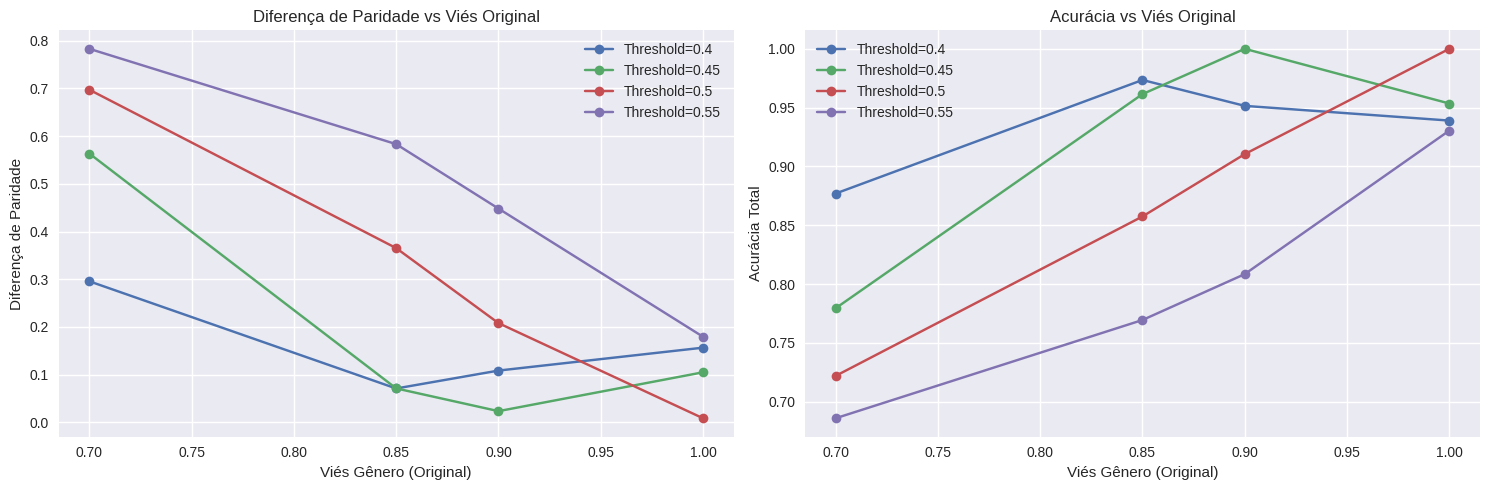
\includegraphics[width=\linewidth]{figs/cel43.png}
\caption{C\'elula 43. Esquerda: DPD $\times$ vi\'es original, uma curva por thr.\ das mulheres. Direita: acur\'acia $\times$ vi\'es.}
\end{figure}

\textbf{Interpreta\c{c}\~ao.} (i) Com thr.\ 0,50 (curva vermelha), o DPD cai de 0,70 (vi\'es 0,7) para $\approx 0$ (vi\'es 1,0) e a acur\'acia sobe de 72\% para 100\%: sem corre\c{c}\~ao, quanto maior o vi\'es, pior o sistema. (ii) Thr.\ baixos compensam o vi\'es: com vi\'es 0,7, passar de 0,50 para 0,40 reduz o DPD de 0,70 para 0,30 e eleva a acur\'acia de 72\% para 88\%. (iii) Corre\c{c}\~ao em excesso prejudica: com vi\'es 1,0, thr.\ 0,40 e 0,45 \textbf{aumentam} o DPD (0,16 e 0,10) e reduzem a acur\'acia (94\% e 95\%), pois se corrige um vi\'es inexistente. (iv) O melhor thr.\ depende do vi\'es: 0,45 para vi\'es 0,9 (DPD 0,023; 100\%), 0,40--0,45 para 0,85 e 0,50 para 1,0. \textit{Ressalva:} cada combina\c{c}\~ao usa amostra aleat\'oria nova (sem \texttt{seed}), logo valores variam entre execu\c{c}\~oes (ex.: vi\'es 1,0/thr.\ 0,50 d\'a DPD 0,009 aqui e 0,035 na c\'elula 48).

\subsection*{B.2 C\'elula 47 --- Taxas de aprova\c{c}\~ao por g\^enero}
\begin{figure}[h]\centering
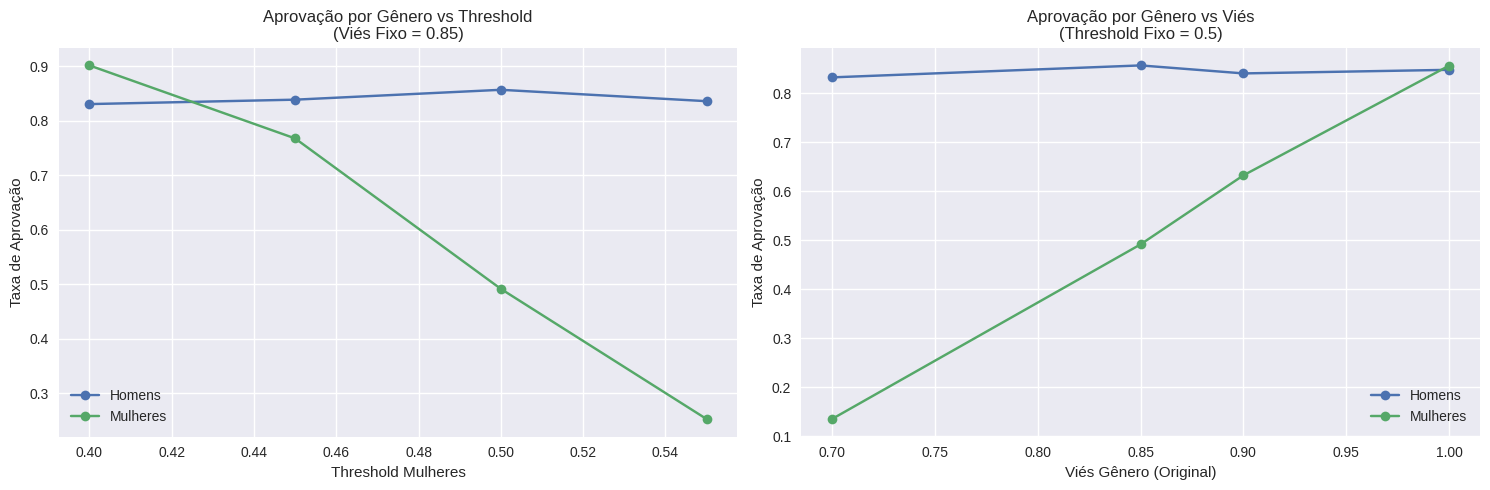
\includegraphics[width=\linewidth]{figs/cel47.png}
\caption{C\'elula 47, a partir da tabela da c\'elula 43. Esquerda: taxas $\times$ thr.\ das mulheres (vi\'es 0,85). Direita: taxas $\times$ vi\'es (thr.\ 0,50).}
\end{figure}

\textbf{Interpreta\c{c}\~ao.} A taxa dos homens fica est\'avel ($\approx$83--86\%), pois o thr.\ masculino e seu \textit{score} n\~ao mudam. Na esquerda, com vi\'es 0,85, a taxa feminina cai de 90,1\% (thr.\ 0,40) para 25,3\% (0,55) e cruza a masculina perto de 0,42: abaixo desse ponto h\'a \textit{sobrecorre\c{c}\~ao} (mulheres aprovadas mais que homens). Na direita, com thr.\ igual para ambos, a taxa feminina sobe de 13,5\% (vi\'es 0,7) para 85,6\% (vi\'es 1,0) e converge \`a masculina: o viés multiplicativo desloca toda a distribui\c{c}\~ao de \textit{scores} das mulheres para baixo, e pequenas penaliza\c{c}\~oes geram quedas grandes porque muitos \textit{scores} ficam pr\'oximos do corte. \textit{Nota:} o texto da c\'elula 45 cita 47,4\%/76,9\%/92,9\%, mas a tabela da c\'elula 43 mostra 49,1\%/76,7\%/90,1\% (thr.\ 0,50/0,45/0,40); os valores variam por falta de \texttt{seed}.

\subsection*{B.3 C\'elula 48 --- Viés 1,0 vs.\ 0,8 (mesma amostra, \texttt{seed}=42)}
\begin{figure}[h]\centering
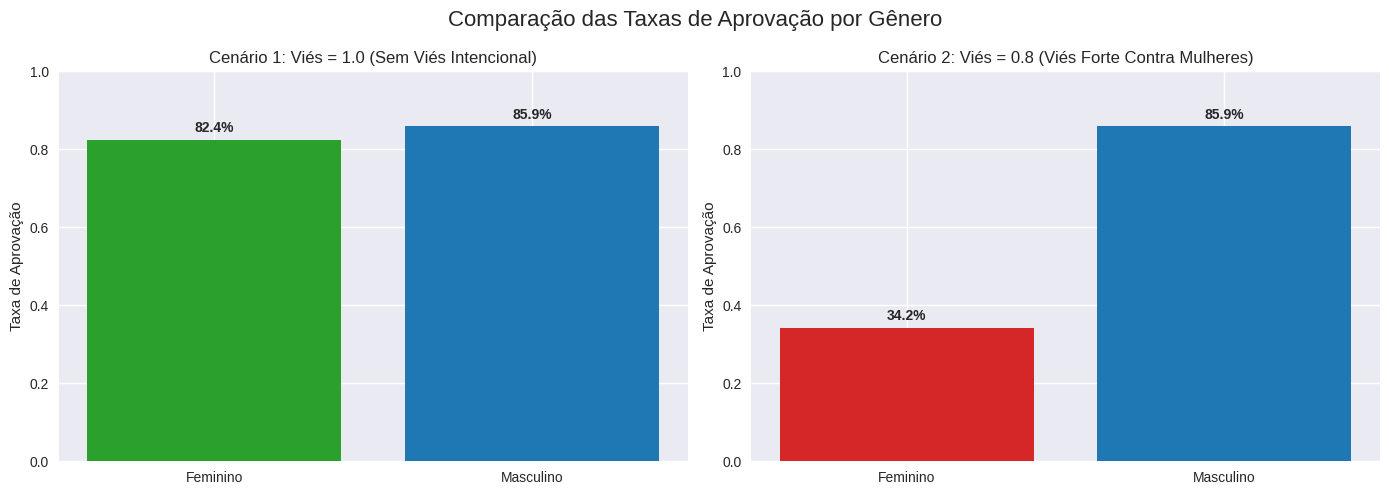
\includegraphics[width=\linewidth]{figs/cel48.png}
\caption{C\'elula 48. Taxas de aprova\c{c}\~ao por g\^enero com vi\'es 1,0 e 0,8 (mesmos clientes, thr.\ 0,50).}
\end{figure}

\textbf{Resultado impresso:} DPD (vi\'es 1,0) = 3,5\%; DPD (vi\'es 0,8) = 51,7\%. Como a \texttt{seed} fixa gera exatamente as mesmas pessoas, a \'unica mudan\c{c}a entre os pain\'eis \'e o fator 0,8 aplicado ao \textit{score} feminino: mulheres passam de 82,4\% para 34,2\% e homens ficam em 85,9\%. Isso isola o efeito do vi\'es. A diferen\c{c}a de 3,5\% no painel esquerdo \'e puro acaso amostral.

\subsection*{B.4 C\'elula 49 --- Trade-off fairness $\times$ acur\'acia (vi\'es 0,8)}
\begin{figure}[h]\centering
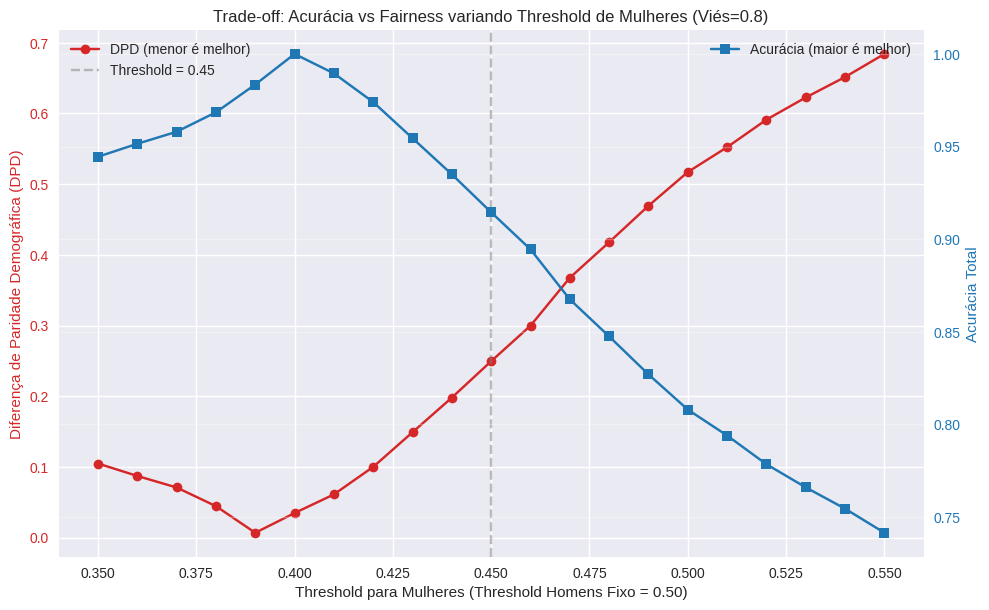
\includegraphics[width=0.78\linewidth]{figs/cel49.png}
\caption{C\'elula 49. DPD (vermelho, eixo esquerdo) e acur\'acia (azul, eixo direito) $\times$ thr.\ das mulheres (0,35--0,55; homens = 0,50).}
\end{figure}

\textbf{Resultado impresso:}
\begin{itemize}
  \item thr.\ 0,50 (sem mitiga\c{c}\~ao): DPD 51,7\%, acur\'acia 80,8\%;
  \item thr.\ 0,45: DPD 25,0\%, acur\'acia 91,5\%;
  \item melhor thr.\ (m\'inimo DPD com acur\'acia $>70\%$) = 0,39: DPD 0,7\%, acur\'acia 98,4\%;
  \item ``Pre\c{c}o'' impresso: $-17{,}5\%$. O sinal negativo indica que a acur\'acia \textbf{aumenta} 17,5 p.p.\ em rela\c{c}\~ao ao modelo sem mitiga\c{c}\~ao; contra o modelo sem vi\'es (100\%), o custo \'e 1,6 p.p.
\end{itemize}
\textbf{Interpreta\c{c}\~ao.} O DPD tem m\'inimo em 0,39 (\textit{valley} da curva vermelha) e a acur\'acia m\'axima (100\%) em 0,40: como $0{,}5\times0{,}8=0{,}4$, o thr.\ 0,40 anula exatamente o vi\'es, e o ponto de DPD m\'inimo difere ligeiramente pela discretiza\c{c}\~ao dos \textit{scores} amostrados. Acima de 0,40 a acur\'acia cai e o DPD cresce quase linearmente; abaixo, ocorre sobrecorre\c{c}\~ao, aprovando mulheres que o \textit{score} base reprovaria. Neste cen\'ario fairness e acur\'acia caminham juntas, porque o ``\textit{ground truth}'' \'e o \textit{score} sem vi\'es.

\end{document}
